% netpoke.tex
%
% Best-effort approximation of the USENIX (NSDI/OSDI/ATC) conference format.
% This does NOT use the official usenix2019/usenix2021 .cls file -- that file
% is distributed by USENIX and was not available to generate this document.
% Before submission, replace the preamble below with the real class:
%   \documentclass[letterpaper,twocolumn,10pt]{article}
%   \usepackage{usenix-2020-09}
% and re-flow this content into its \begin{document}...\end{document}.
% Everything from \begin{document} onward (title, sections, tables, figures,
% bibliography) should carry over with minimal changes.

\documentclass[letterpaper,twocolumn,10pt]{article}
\usepackage[letterpaper,margin=0.75in,columnsep=0.3in]{geometry}
\usepackage{times}
\usepackage{graphicx}
\usepackage{booktabs}
\usepackage{amsmath}
\usepackage{url}
\usepackage{hyperref}
\usepackage{pgfplots}
\pgfplotsset{compat=1.17}
\usepackage{titlesec}
\usepackage{caption}

\titleformat{\section}{\normalfont\large\bfseries}{\thesection}{1em}{}
\titleformat{\subsection}{\normalfont\bfseries}{\thesubsection}{1em}{}
\captionsetup{font=small,labelfont=bf}

\title{\Large\bfseries NetPoke: Restoring Causal-Profiling Accuracy \\ for I/O-Bound Microservices}

\author{
Afram Visca Gyebi \\
\small Kwame Nkrumah University of Science and Technology \\
\small \texttt{[institutional email]}
}
\date{}

\begin{document}
\twocolumn[
\maketitle
\begin{abstract}
\noindent
SlowPoke predicts the end-to-end throughput impact of hypothetical service
optimisations in microservice applications by pausing non-target services
with \texttt{SIGSTOP} and measuring the resulting slowdown. This causal
approach avoids the need for distributed tracing or prior knowledge of the
service call graph, and it is accurate for CPU-bound services. It is less
accurate for I/O-bound ones, because \texttt{SIGSTOP} halts a process's
scheduling but not the kernel's handling of that process's open network
connections: data destined for a paused service is still accepted into
kernel buffers and arrives as a burst the moment the process resumes,
polluting the measurement the pause was meant to produce cleanly. We
measure this gap directly on a cluster reproduction of SlowPoke's own
evaluation, finding baseline prediction error ranging from 2.57\% for a
target with no synchronous network I/O to over 20\% for targets with real
downstream dependencies. We present NetPoke, a network-layer mitigation
that holds a paused service's egress traffic for exactly the duration of
each real \texttt{SIGSTOP}/\texttt{SIGCONT} pair, implemented as a Linux
\texttt{sch\_plug} queueing discipline driven directly from SlowPoke's own
pause controller over a netlink control channel. Across four benchmark
applications, NetPoke reduces residual network I/O crossing pause windows
by a factor of 2.2 to 4.3 for the three applications whose targets perform
synchronous I/O, and this translates into restored prediction accuracy,
most substantially a 76\% recovery of lost accuracy for one application. For
the fourth application, whose target performs no synchronous I/O in its
live request path, NetPoke provides no benefit and a small, measurable
cost, a result we trace to a specific, verifiable property of that
application's source code rather than leave unexplained.
\end{abstract}
\vspace{1em}
]

\section{Introduction}

Deciding which service to optimise in a microservice application is a
resource-allocation problem before it is an engineering one. A team with
limited time has to guess which candidate optimisation will actually move
the end-to-end throughput number that matters to users and operators, and
guessing wrong wastes the time spent implementing an optimisation that
turns out not to matter. Causal profiling answers this question by
measurement rather than guesswork: instead of building the optimisation to
see if it helps, deliberately slow down everything else and observe how
much the target's relative contribution to overall throughput actually is.

SlowPoke~\cite{slowpoke2026} brought this technique, first developed for
single-machine multithreaded programs by Coz~\cite{coz2015}, to distributed
microservice applications. It slows down non-target services using
\texttt{SIGSTOP}, an uncatchable POSIX signal that removes a process from
the CPU scheduler, and predicts the throughput of a hypothetical
optimisation from the resulting measurement using a closed-form performance
model. Evaluated across real-world benchmark applications, SlowPoke reports
a root-mean-squared prediction error of 2.07\%.

That accuracy depends on an assumption the SlowPoke paper itself identifies
as fragile: that pausing a service with \texttt{SIGSTOP} produces a
bottleneck-equivalent execution to the one a real optimisation would
produce. This holds for CPU-bound services, where halting scheduling
directly halts progress. It does not hold cleanly for services whose
bottleneck is synchronous network I/O, because \texttt{SIGSTOP} controls
scheduling, not the kernel's network stack. A packet destined for a paused
process's socket still arrives, still gets acknowledged, and still sits in
a receive buffer waiting for a \texttt{read()} call that will not happen
until the process resumes. The SlowPoke paper acknowledges this limitation
in its own discussion of future work but neither measures its size nor
proposes and evaluates a fix.

This paper does both. We first measure the gap directly, on a cluster
reproduction of SlowPoke's own evaluation methodology (\S\ref{sec:motivation}).
We then present NetPoke, a network-layer mitigation that closes it
(\S\ref{sec:design}, \S\ref{sec:implementation}), and evaluate it against
the same benchmark applications used to characterise the original problem
(\S\ref{sec:evaluation}). We make the following contributions:

\begin{itemize}
\item A direct, cluster-based measurement of SlowPoke's accuracy gap
  between CPU-bound and I/O-bound causal targets, using both an indirect
  injection-based method and a direct in-pod residual-I/O measurement that
  resolves a case where the two disagree.
\item NetPoke, a network egress hold integrated directly into SlowPoke's
  own pause controller via a Linux \texttt{sch\_plug} queueing discipline,
  synchronised to real pause events over a netlink control channel rather
  than driven by a separately configured delay.
\item An evaluation showing NetPoke reduces residual I/O by 2.2--4.3$\times$
  and restores prediction accuracy for three of four benchmark applications,
  including a 76\% recovery of lost accuracy for the application with the
  clearest I/O-bound signal.
\item A source-level explanation, not merely an empirical observation, of
  the one case where NetPoke does not help: a target with no synchronous
  network I/O in its live request-handling code gains nothing and pays a
  small, measurable, consistent cost instead.
\end{itemize}

\section{Background and Motivation}
\label{sec:motivation}

\subsection{SlowPoke and POKER}

SlowPoke's performance model rests on bottleneck equivalence: if
non-target services are paused for precisely the amount of time a
hypothetical optimisation would have removed from the target, the paused
system's throughput reveals what the optimised system's throughput would
be, without building the optimisation. The pause duration for each
non-target service is computed from the target's request ratio and each
service's relative CPU allocation, and applied by \texttt{poker}, a small
control process co-located with each service, using \texttt{SIGSTOP} and
\texttt{SIGCONT} on the service's process group.

\texttt{SIGSTOP} is precise about what it controls. It removes a process
from the kernel's CPU scheduler; the process is guaranteed not to run
again until \texttt{SIGCONT}. It does not affect the kernel's own handling
of that process's open sockets, which continues via interrupt-driven
processing independent of whether the owning process is scheduled. For a
CPU-bound target, no meaningful I/O happens during a pause regardless, so
this distinction is immaterial. For a service whose work involves waiting
on a database query or a call to another service, it is not: data can
arrive and be acknowledged throughout the pause, then processed in a
burst the instant the process resumes, work the hypothetical optimisation
never removed.

\subsection{Measuring the Gap}
\label{sec:measuring-gap}

We reproduce SlowPoke's own evaluation on an eight-node Kubernetes cluster
using SlowPoke's own artifact and four benchmark applications: Online
Boutique~\cite{onlineboutique}, an independently maintained e-commerce
demo (target service: \texttt{cart}), and three DeathStarBench
applications~\cite{deathstarbench2019}: hotel reservation (target:
\texttt{profile}), social network (target: \texttt{hometimeline}), and a
media review service (target: \texttt{moviereviews}).

\begin{table}[t]
\centering
\small
\caption{Baseline prediction accuracy, no injection.}
\label{tab:baseline}
\begin{tabular}{lcc}
\toprule
App & Target & RMSE (\%) \\
\midrule
Boutique & cart & 2.57 \\
Hotel & profile & 20.65 \\
Social & hometimeline & 14.01 \\
Movie & moviereviews & 12.21 \\
\bottomrule
\end{tabular}
\end{table}

Table~\ref{tab:baseline} shows substantial variation even with no
additional I/O stress: boutique's cart target closely reproduces the
paper's own reported 2.07\% accuracy, while the other three targets, all
of which have real downstream service or state-store dependencies (\S
\ref{sec:evaluation}), show markedly higher baseline error. Deliberately
adding synchronous-I/O delay to the path downstream of each target, using
\texttt{netem}, pushes social network's error up by a further 19.6
percentage points, the cleanest single signal in our data that the
mechanism SlowPoke's authors flagged as a limitation is a real,
measurable effect, not merely a theoretical one. Not every application's
result is as clean; we return to this, and to a direct instrument that
resolves a contradictory result for hotel, in \S\ref{sec:evaluation}.

\section{Design}
\label{sec:design}

NetPoke's design goal follows directly from the mechanism identified in \S
\ref{sec:motivation}: a service's network activity should stop for exactly
as long as its process is stopped, and resume exactly when the process
resumes, without requiring application code changes or a separate process
in the deployment.

An earlier design, considered and set aside during this project, used a
sidecar container applying a fixed, pre-configured \texttt{netem} delay to
incoming traffic. We rejected this approach for two reasons. First,
\texttt{poker}'s actual pause durations vary per invocation, computed from
the performance model and from batching, so a statically configured delay
can only approximate the real window, not match it. Second, running the
hold in a process separate from \texttt{poker} requires synchronising two
independently scheduled programs across a process boundary, reintroducing
timing slack the mechanism exists to eliminate.

NetPoke instead holds a service's egress traffic using the Linux
\texttt{sch\_plug} queueing discipline, installed as the root \texttt{tc}
qdisc on the service's network interface. This discipline, originally
built to buffer traffic during virtual-machine live migration, exposes a
buffer action and a release action that map directly onto pause start and
pause end. Critically, we drive it from inside \texttt{poker} itself,
immediately before the existing \texttt{SIGSTOP} call and immediately
after the existing \texttt{SIGCONT} call, so the hold is synchronised to
the pause controller's own knowledge of real pause boundaries rather than
to a separately maintained estimate of them.

\section{Implementation}
\label{sec:implementation}

\texttt{poker} opens a single \texttt{AF\_NETLINK} socket over the
\texttt{NETLINK\_ROUTE} protocol family at startup, the same kernel
interface used internally by \texttt{tc} and \texttt{ip}. Toggling the
hold is a single message on this socket, addressed to the previously
installed \texttt{sch\_plug} qdisc at the interface root, carrying a
kernel data structure (\texttt{struct tc\_plug\_qopt}) with an action code
and a buffer limit. Because the socket is held open for the pod's
lifetime rather than reopened per toggle, each toggle costs on the order
of microseconds.

Two implementation issues were significant enough to be worth recording.
The kernel initially rejected every toggle message with \texttt{EINVAL};
the cause was that \texttt{sch\_plug} expects \texttt{struct
tc\_plug\_qopt} written directly as the netlink options payload, not
wrapped in a nested routing attribute as most other \texttt{tc} options
are encoded, and correcting this required a full rewrite of the
message-encoding path. Separately, the netlink \texttt{recvmsg()} call
used to confirm a toggle had no timeout, so a lost or malformed
acknowledgement could block the pause loop indefinitely; we added a
100ms \texttt{SO\_RCVTIMEO} to bound this failure mode.

To make the results in \S\ref{sec:evaluation} possible to measure at all,
we also added unconditional pause-window logging to \texttt{poker} itself,
printing a timestamped marker at the start and end of every pause
regardless of whether NetPoke is enabled. Without this, a SIGSTOP-only run
produces no record of when its pause windows actually occurred, making it
impossible to establish a genuine baseline for comparison.

\section{Evaluation}
\label{sec:evaluation}

We evaluate NetPoke in three stages: a direct, in-pod measurement of
residual network I/O crossing real pause windows; an end-to-end
prediction-accuracy comparison under injected I/O stress; and the same
accuracy comparison with no injection, to test whether NetPoke's cost is
specific to the injected-stress condition.

\subsection{Residual I/O}

We built an in-pod sampler that polls per-process and per-interface I/O
counters (\texttt{/proc/[pid]/io}, \texttt{/proc/net/dev}) at a
10ms interval, correlated against \texttt{poker}'s own pause-window
markers, and report residual I/O as the ratio of bytes received during
pause windows to bytes received outside them.

\begin{table}[t]
\centering
\small
\caption{Residual I/O (L2, injected condition), SIGSTOP-only vs.\ NetPoke-on.}
\label{tab:residual}
\begin{tabular}{lccc}
\toprule
App & SIGSTOP-only & NetPoke-on & Reduction \\
\midrule
Boutique & 3.28\% & 4.28\% & none \\
Hotel & 9.52\% & 3.33\% & 2.9$\times$ \\
Social & 8.91\% & 4.00\% & 2.2$\times$ \\
Movie & 6.89\% & 1.59\% & 4.3$\times$ \\
\bottomrule
\end{tabular}
\end{table}

Table~\ref{tab:residual} shows a substantial reduction for three of four
applications. This measurement is also what resolves a discrepancy in our
injection-based results (\S\ref{sec:accuracy}): hotel's accuracy under
\texttt{netem} injection contradicted the I/O-gap hypothesis, decreasing
rather than increasing with more injected I/O, but hotel's direct
residual-I/O measurement here is unremarkable, in the same range as social
and movie. We treat the direct measurement as the more trustworthy signal
and the injection-based accuracy method as a noisier proxy of the
underlying phenomenon.

\subsection{Prediction Accuracy}
\label{sec:accuracy}

\begin{figure}[t]
\centering
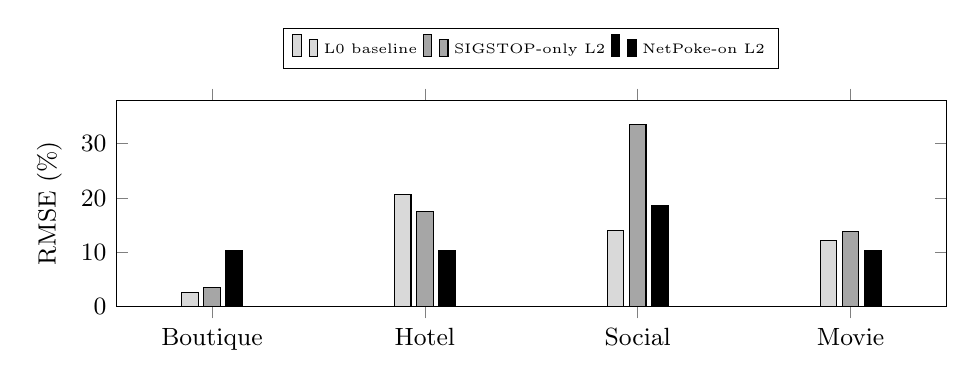
\begin{tikzpicture}
\begin{axis}[
  ybar, bar width=6pt, width=\linewidth, height=4.2cm,
  ylabel={RMSE (\%)}, ylabel style={font=\small},
  symbolic x coords={Boutique,Hotel,Social,Movie},
  xtick=data, tick label style={font=\small},
  ymin=0, ymax=38,
  legend style={font=\tiny, at={(0.5,1.15)}, anchor=south, legend columns=3},
  enlarge x limits=0.15,
]
\addplot[fill=gray!30] coordinates {(Boutique,2.57) (Hotel,20.65) (Social,14.01) (Movie,12.21)};
\addplot[fill=gray!70] coordinates {(Boutique,3.53) (Hotel,17.51) (Social,33.61) (Movie,13.84)};
\addplot[fill=black] coordinates {(Boutique,10.26) (Hotel,10.25) (Social,18.69) (Movie,10.23)};
\legend{L0 baseline, SIGSTOP-only L2, NetPoke-on L2}
\end{axis}
\end{tikzpicture}
\caption{End-to-end prediction RMSE: no-injection baseline, injected I/O
  stress without NetPoke, and injected I/O stress with NetPoke.}
\label{fig:rmse}
\end{figure}

We repeat SlowPoke's ten-point accuracy benchmark at the injected-stress
condition (L2) with NetPoke enabled and compare against the SIGSTOP-only
L2 numbers (Figure~\ref{fig:rmse}). Social network, the application with
the clearest I/O-gap signal in \S\ref{sec:measuring-gap}, sees RMSE fall
from 33.61\% to 18.69\%, recovering 76\% of the gap between the injected
and no-injection baselines. Hotel and movie also improve, both ending at
or below their own L0 baselines. Boutique gets worse, from 3.53\% to
10.26\%.

We repeat the same accuracy comparison at L0, with no injection at all,
to test whether boutique's regression is specific to the injected
condition. It is not: boutique's L0 RMSE rises from 2.57\% to 9.13\% with
NetPoke on, a 6.56 percentage-point increase, close to its 6.73
percentage-point increase at L2. Two independently run experiments
arriving at a similar magnitude is stronger evidence of a real, consistent
cost than either result alone.

\subsection{Explaining Boutique}

\begin{table}[t]
\centering
\small
\caption{Network I/O in each target's live request-handling code.}
\label{tab:fanout}
\begin{tabular}{lp{5.2cm}}
\toprule
App & Live-path network calls \\
\midrule
Boutique & None (in-process map only; unused Redis/state code present) \\
Hotel & State-store round trip \\
Movie & State-store round trip + call to \texttt{reviewstorage} \\
Social & State-store round trip + call to \texttt{poststorage} \\
\bottomrule
\end{tabular}
\end{table}

We traced boutique's target directly in source (Table~\ref{tab:fanout}).
Its handler operates entirely on an in-process map; a Redis client and a
state-store call exist in the same file but are not reached by the code
path the benchmark exercises. The other three targets each perform at
least one genuine network round trip. Boutique's target has no residual
I/O for NetPoke to intercept, which is consistent with Table
\ref{tab:residual}, and NetPoke's real per-toggle cost (\S
\ref{sec:implementation}) has nothing to offset it, which explains the
regression rather than leaving it as an anomaly.

\section{Related Work}

Causal profiling originates with Coz~\cite{coz2015}, which applies the
same slow-everything-else-and-measure technique within a single
multithreaded process. SlowPoke~\cite{slowpoke2026} is, to our knowledge,
the first system to extend this technique across process and machine
boundaries to distributed microservice applications; NetPoke extends
SlowPoke's own mechanism rather than proposing an alternative causal-profiling
approach. Distributed tracing systems such as Dapper~\cite{dapper2010}
take a different, diagnostic approach: they reconstruct where time was
spent on completed requests rather than predicting the effect of a
hypothetical change, and answering a what-if question from trace data
alone requires a separate predictive model layered on top. DeathStarBench
\cite{deathstarbench2019} provides the realistic, independently maintained
benchmark applications used throughout our evaluation.

\section{Discussion and Limitations}

All measurements in this paper are single runs per application per
condition rather than averages over repeated trials; hotel's baseline RMSE
alone moved by roughly ten percentage points between two runs collected
under nominally identical conditions with no experimental manipulation
applied, which sets a lower bound on how much weight any single-run result
on our cluster can bear. Boutique's regression is the exception: measured
independently under two conditions (injected and no-injection) and landing
within 0.2 percentage points of itself both times, it is better supported
than a single-run result would be. NetPoke addresses network I/O only;
disk I/O buffering is a related but distinct failure mode and is out of
scope. The practical implication of boutique's result is that NetPoke
should not be enabled unconditionally on every service in a deployment; a
mechanism to identify, before enabling NetPoke, whether a target's live
request path performs synchronous network I/O at all would let it be
applied selectively. We did not build such a mechanism and identify it as
future work.

\section{Conclusion}

NetPoke closes a gap SlowPoke's own authors identified but did not measure
or address: a network-layer egress hold, driven directly from SlowPoke's
pause controller and synchronised to real pause events rather than a
configured delay, reduces residual I/O crossing pause windows by 2.2 to
4.3$\times$ and restores prediction accuracy, including a 76\% recovery
for the application with the clearest I/O-bound signal in our evaluation.
Where a target has no synchronous I/O to begin with, NetPoke provides no
benefit and a small, traceable cost rather than an unexplained regression,
a boundary this paper establishes with source-level evidence rather than
leaves as an open question.

\begin{thebibliography}{9}

\bibitem{slowpoke2026}
Y.~Xie, D.~Jin, O.~{\c C}{\"o}lkesen, V.~Kalavri, J.~Liagouris, and
N.~Vasilakis.
\newblock Slowpoke: End-to-end Throughput Optimization Modeling for
  Microservice Applications.
\newblock In \emph{23rd USENIX Symposium on Networked Systems Design and
  Implementation (NSDI 26)}, Renton, WA, 2026. USENIX Association.

\bibitem{coz2015}
C.~Curtsinger and E.~D. Berger.
\newblock Coz: Finding Code that Counts with Causal Profiling.
\newblock In \emph{Proceedings of the 25th Symposium on Operating Systems
  Principles (SOSP)}, 2015.

\bibitem{deathstarbench2019}
Y.~Gan et al.
\newblock An Open-Source Benchmark Suite for Microservices and Their
  Hardware-Software Implications for Cloud \& Edge Systems.
\newblock In \emph{Proceedings of the Twenty-Fourth International
  Conference on Architectural Support for Programming Languages and
  Operating Systems (ASPLOS)}, 2019.

\bibitem{dapper2010}
B.~H. Sigelman et al.
\newblock Dapper, a Large-Scale Distributed Systems Tracing Infrastructure.
\newblock Google Technical Report dapper-2010-1, 2010.

\bibitem{onlineboutique}
Google Cloud Platform.
\newblock Online Boutique: Cloud-Native Microservices Demo Application.
\newblock \url{https://github.com/GoogleCloudPlatform/microservices-demo}.

\end{thebibliography}

\end{document}
